\documentclass[
  bibliography=totoc,     % Literatur im Inhaltsverzeichnis
  captions=tableheading,  % Tabellenüberschriften
  titlepage=firstiscover, % Titelseite ist Deckblatt
]{scrartcl}

% Paket float verbessern
\usepackage{scrhack}

% Warnung, falls nochmal kompiliert werden muss
\usepackage[aux]{rerunfilecheck}

% unverzichtbare Mathe-Befehle
\usepackage{amsmath}
% viele Mathe-Symbole
\usepackage{amssymb}
% Erweiterungen für amsmath
\usepackage{mathtools}

% Fonteinstellungen
\usepackage{fontspec}
% Latin Modern Fonts werden automatisch geladen
% Alternativ zum Beispiel:
%\setromanfont{Libertinus Serif}
%\setsansfont{Libertinus Sans}
%\setmonofont{Libertinus Mono}

% Wenn man andere Schriftarten gesetzt hat,
% sollte man das Seiten-Layout neu berechnen lassen
\recalctypearea{}

% deutsche Spracheinstellungen
\usepackage[ngerman]{babel}


\usepackage[
  math-style=ISO,    % ┐
  bold-style=ISO,    % │
  sans-style=italic, % │ ISO-Standard folgen
  nabla=upright,     % │
  partial=upright,   % ┘
  warnings-off={           % ┐
    mathtools-colon,       % │ unnötige Warnungen ausschalten
    mathtools-overbracket, % │
  },                       % ┘
]{unicode-math}

% traditionelle Fonts für Mathematik
\setmathfont{Latin Modern Math}
% Alternativ zum Beispiel:
%\setmathfont{Libertinus Math}

\setmathfont{XITS Math}[range={scr, bfscr}]
\setmathfont{XITS Math}[range={cal, bfcal}, StylisticSet=1]

% Zahlen und Einheiten
\usepackage[
  locale=DE,                   % deutsche Einstellungen
  separate-uncertainty=true,   % immer Unsicherheit mit \pm
  per-mode=symbol-or-fraction, % / in inline math, fraction in display math
]{siunitx}

% chemische Formeln
\usepackage[
  version=4,
  math-greek=default, % ┐ mit unicode-math zusammenarbeiten
  text-greek=default, % ┘
]{mhchem}

% richtige Anführungszeichen
\usepackage[autostyle]{csquotes}

% schöne Brüche im Text
\usepackage{xfrac}

% Standardplatzierung für Floats einstellen
\usepackage{float}
\floatplacement{figure}{htbp}
\floatplacement{table}{htbp}

% Floats innerhalb einer Section halten
\usepackage[
  section, % Floats innerhalb der Section halten
  below,   % unterhalb der Section aber auf der selben Seite ist ok
]{placeins}

% Seite drehen für breite Tabellen: landscape Umgebung
\usepackage{pdflscape}

% Captions schöner machen.
\usepackage[
  labelfont=bf,        % Tabelle x: Abbildung y: ist jetzt fett
  font=small,          % Schrift etwas kleiner als Dokument
  width=0.9\textwidth, % maximale Breite einer Caption schmaler
]{caption}
% subfigure, subtable, subref
\usepackage{subcaption}

% Grafiken können eingebunden werden
\usepackage{graphicx}

% schöne Tabellen
\usepackage{booktabs}

% Verbesserungen am Schriftbild
\usepackage{microtype}

% Literaturverzeichnis
\usepackage[
  backend=biber,
]{biblatex}
% Quellendatenbank
\addbibresource{lit.bib}
%\addbibresource{programme.bib}

% Hyperlinks im Dokument
\usepackage[
  german,
  unicode,        % Unicode in PDF-Attributen erlauben
  pdfusetitle,    % Titel, Autoren und Datum als PDF-Attribute
  pdfcreator={},  % ┐ PDF-Attribute säubern
  pdfproducer={}, % ┘
]{hyperref}
% erweiterte Bookmarks im PDF
\usepackage{bookmark}

% Trennung von Wörtern mit Strichen
\usepackage[shortcuts]{extdash}

\author{
  Thomas-Christopher Ogasa \\
  \href{mailto:thomas.ogasa@tu-dortmund.de}{thomas.ogasa@tu-dortmund.de}
  \\
  \\
  Jiayue Ruan \\
  \href{mailto:jiayue.ruan@tu-dortmund.de}{jiayue.ruan@tu-dortmund.de}
}
\publishers{TU Dortmund – Fakultät Physik}

\renewcommand{\d}{\symup{d}}
\newcommand{\diff}[2]{\frac{\symup{d} #1}{\symup{d} #2}}
\newcommand{\e}{\symup{e}}
\newcommand{\idx}[1]{_{\symup{ #1 }}}
\newcommand{\pdiff}[2]{\frac{\partial #1}{\partial #2}}

\subject{V47}
\title{Molar heat capacity of copper}
\date{
  Durchführung: 26.06.2023
}
\usepackage[aux]{rerunfilecheck}

\usepackage{fontspec}
\usepackage{siunitx}

\usepackage[ngerman]{babel}

\usepackage[unicode]{hyperref}
\usepackage{bookmark}
\usepackage{booktabs}
\usepackage{import}
\usepackage{amsmath}

\usepackage{scrhack}

\usepackage[aux]{rerunfilecheck}

\usepackage{fontspec}

\usepackage[ngerman]{babel}

\usepackage{amsmath}
\usepackage{amssymb}
\usepackage{mathtools}

\usepackage{booktabs}

\usepackage[unicode]{hyperref}
\usepackage{bookmark}
\usepackage{svg}

\begin{document}

\maketitle
\thispagestyle{empty}
\tableofcontents
\newpage


\section{Goal}
In this experiment the specific heat capacity of copper as well as the debye temperature. Further the temperature dependence of the 
heat capacity will be compared to the theoretical predictions of the debye model.
\section{Theory}
There are 3 commonly used theories to describe the specific heat capacity. The classical approach, the Einstein model and the Debye model.
Each approach will be explained in the following.
\subsection{Classical predictions of the specific heat capacity}
In classical thermodynamics, the expected kinetic energy of a particle can be expressed as 
\begin{equation*}
    <u\idx{i}> = \frac{1}{2}k\idx{B}T
\end{equation*}
per positional degree of freedom of the particle, with $k\idx{B}$ being the Boltzmann constant and $T$ being the temperature. In generall
a particle has 3 positional degrees of freedom so a mean energy of 
\begin{equation*}
    <u\idx{i}> = \frac{3}{2}k\idx{B}T.
\end{equation*}
According to the Virial theorem the mean potential energy and mean kinetic energy of a harmonic oscillator is the same. The specific heat 
capacity of a solid, consisting of $N$ particles, is defined as
\begin{equation*}
    C\idx{V} = \frac{\delta U}{\delta T} = \frac{\delta 3\cdot Nk\idx{B}T}{\delta T} = 3\cdot Nk\idx{B}.
\end{equation*}
$C\idx{V}$ in this case is the heat capacity with constant volume. For solids it is often easier to measure the heat capacity at 
constant pressure, or $C\idx{p}$, which is related to the former via
\begin{equation}
    C\idx{p}-C\idx{V} = VT\frac{\alpha^2}{\beta},
    \label{eq:CpCV}
\end{equation}
with $V$ being the volume $\alpha$ the thermal expansion coefficient and $\beta$ the compressibility.
\subsection{Einstein model}
In the Einstein model, the quantization of vibrational energies and frequencies of individual atoms in a solid is considered. It assumes 
that all oscillators vibrate at the same frequency $\omega$, and their energies being multiples of $\hbar\omega$, where 
$\hbar$ represents the reduced Planck's constant. The probability, $W(n)$, of an oscillator having an energy equal to $n\hbar\omega$ 
at a given temperature $T$ is described by the Boltzmann distribution:
\begin{equation*}
W(n) = \exp\left(-\frac{n\hbar\omega}{k\idx{B}T}\right)
\end{equation*}
The average energy per atom, $<u>\idx{Einstein}$, is calculated by summing over all possible energies, $n\hbar\omega$, weighted by their 
respective probabilities, and dividing by the sum of all $W(n)$:
\begin{equation*}
<u>\idx{Einstein} = \frac{\sum_{n=0}^{\infty}n\hbar\omega W(n)}{\sum_{n=0}^{\infty}W(n)} = \frac{\hbar\omega}{\exp\left(\frac{\hbar\omega}{k\idx{B}T}\right)-1} 
\end{equation*}
The molar heat capacity at constant volume, $C\idx{V}$, can be calculated by differentiating the average energy with respect to temperature, 
like in the classical case, resulting in 
\begin{equation*}
C\idx{V, Einstein} = \frac{3R(\frac{\hbar\omega}{k\idx{B}T})^{2}\exp(\frac{\hbar\omega}{k\idx{B}T})}{(\exp(\frac{\hbar\omega}{k\idx{B}T})-1s)^{2}}.
\end{equation*}
For high temperatures it converges on the classical prediction of $3Nk\idx{B}$
\subsection{Debye model}
The Debye model takes into account the distribution of vibrational frequencies in a solid, rather than assuming a single frequency for all 
oscillators. It introduces a characteristic frequency called the Debye frequency, denoted as $\omega\idx{D}$, which represents the maximum 
frequency of vibrations in the solid. The energy levels of the vibrational modes are quantized in units of $\hbar\omega$, and the Debye model 
considers an integration over all possible frequencies weighted by the density of states function, $D(\omega)$. The average energy per atom 
in the Debye model, $<u>\idx{Debye}$, is given by:
\begin{equation*}
 <u>\idx{Debye} = 9Nk\idx{B}T \left(\frac{T}{\Theta\idx{D}}\right)^3\int_{0}^{\Theta\idx{D}/T} \frac{x^3}{\exp(x)-1} dx 
\end{equation*}
where $\Theta\idx{D} = \frac{\hbar\omega\idx{D}}{k\idx{B}}$ is the Debye temperature.

The molar heat capacity at constant volume, $C\idx{V}$, in the Debye model can be obtained by differentiating the average energy with 
respect to temperature:
\begin{equation*}
    C\idx{V, Debye} = 9R\left(\frac{T}{\Theta\idx{D}}\right)^3\int_{0}^{\Theta\idx{D}/T} \frac{x^4\exp(x)}{(\exp(x)-1)^2} dx
\end{equation*}
The Debye model provides a better description of the specific heat capacity of solids at low temperatures compared to the Einstein model. 
However, it also has limitations, such as assuming a linear sound velocity and neglecting anharmonicity effects.
 


\section{Setup and Procedure}
\begin{figure}[h]
    \centering
    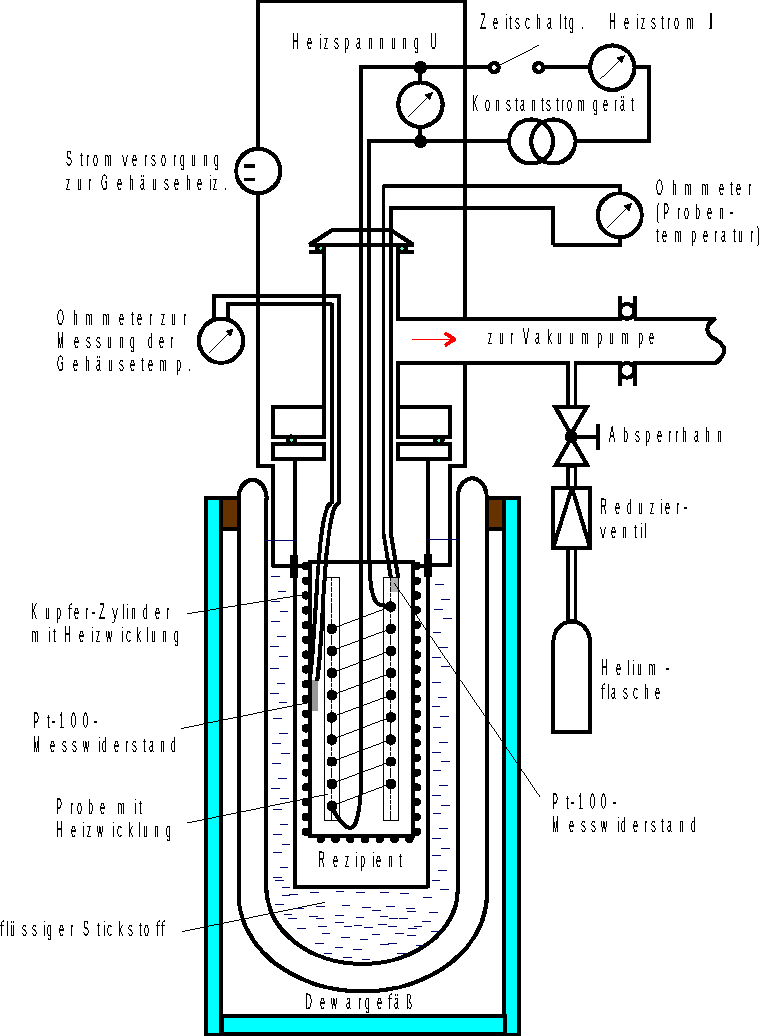
\includegraphics[scale=0.65]{Aufbau.pdf}
    \caption{Setup of the experiment \cite{V47}.}
    \label{fig:aufbau}
\end{figure}
The experimental setup for determining the specific heat of copper is housed in a Dewar flask filled with liquid nitrogen to ensure the 
required temperature range for this experiment. Inside the Dewar flask is the copper sample, which is surrounded by heating coils. The 
energy added by the heating coils to the sample and the temperature profile of the sample are measured during the experiment. The energy 
input is measured using the voltage and current with which the heating coils are operated, along with the time interval between two measurement 
points. The temperature of the sample is measured using the resistance of a PT-100 probe. To prevent heat losses through convection and heat 
conduction, a chamber enclosing the sample is evacuated for the measurement. Furthermore, a copper cylinder is positioned around the sample, 
which is ideally heated to the same temperature using another heating mantle to minimize radiative losses. The aforementioned quantities are 
measured at specific temperatures ranging from $80$ to $\SI{300}{\kelvin}$.


\section{Auswertung}



\section{Diskussion}





\nocite{*}
\printbibliography

\newpage
\addsec{Anhang}


\end{document}
